\chapter{Implementation}
\label{ch:impl}
In the first part of this chapter we describe the recognition system implemented by this thesis, in the second part we describe the game prototype that demonstrates the usage of the algorithm. Implementation of the recognition system consists of two parts, one responsible for the actual recognition, and one for the training of neural network based on user-defined shapes. The usage of the framework consists of three steps:
\begin{enumerate}
\item Defining the shapes and setting up desired recognition parameters.
\item Training the neural network to classify the defined shapes.
\item Using the framework and the trained network to recognize patterns.
\end{enumerate}

\section{Data representations}
We have developed several data classes that are crucial for the algorithm functionality. The \texttt{ImageLines} is a class that holds the input to the algorithm. The next class is a \texttt{ShapeDescriptor}, an abstract class whose implementations are used to describe shapes, and the last one is a \texttt{ShapeNode} class for the output data representation.

\begin{description}
\item [Image lines class]
We use the vector form in the interface. The shapes are defined as a vector of lines with the start and end point.
The format of input is an instance of the \texttt{ImageLines} class, defined in the \texttt{ImageAnalyzer.h} header file. This class wraps a vector of lines defining the shape, accessible through \texttt{GetImageLines} method. The user is expected to fill the vector with the lines representing the two-dimensional image before passing it into the \texttt{Analyze} method. The class offers several other methods, used primarily by the recognition algorithm. 

A line is represented by the instance of class \texttt{Line}, whose constructor accepts two \texttt{float2} type vectors, first containing the start coordinates of the line, and second containing the end coordinates. Internally, the coordinates are transformed into three-dimensional vectors of a homogeneous coordinate system. 

\item [Shape descriptors]
Shape descriptors are a key part of the system, as they are used both during training of the neural network and during analysis of image. They provide the information about the expected line positions and possible embedded shape locations to the algorithm.

Library user can define their own shapes by inheriting from the abstract class \texttt{ShapeDescriptor} defined in \texttt{ImageAnalyzer.h} file. The shape descriptors use the parametric-like expressions to define shapes. Abstract class functions, which should be defined by the user, take parameter \texttt{t} in the interval $[0,1]$ as an argument, and return a point on the curve in a 2D space in the interval $[0,1]^2$.

The curve does not have to be continuous, but it has to return a value for every parameter value in the range. Thread safety of some methods is also required. It is recommended to keep the shape complexity low, as some very small details may be lost in the data preparation for the training.

\item [Output data format]
Output of the algorithm implementation is in the form of instance of \texttt{ShapeNode} class defined in \texttt{ImageAnalyzer.h} file. It represents a tree structure shown in \cref{fig:output0}, where each node contains the recognized shape index and its pattern shape index. Embedded shapes are contained in a vector of child nodes. Indexes are numbers assigned to each descriptor during algorithm setup, except for the \texttt{unknown} shape index, which serves as a placeholder for unrecognized shapes. We do not differentiate between the empty space and any unrecognized shape.

\begin{figure}[p]
\centering
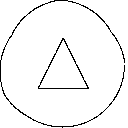
\includegraphics[width=.3\linewidth]{ext/images/example_output0.png}
\quad
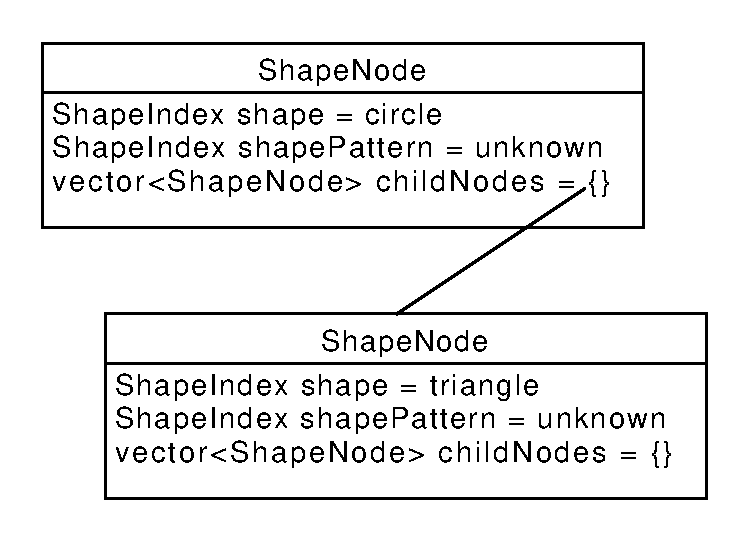
\includegraphics[width=.3\linewidth]{ext/images/example_output0.pdf}
\caption{Input image with expected output. The embeddings form a tree hierarchy, with a single shape in the root and it's embedded shapes as its sons. The \texttt{unknown} shape index marks both unrecognized shapes and empty space.}
\label{fig:output0}
\end{figure}

\begin{figure}[p]
\centering
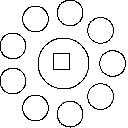
\includegraphics[width=.3\linewidth]{ext/images/example_output1.png}
\quad
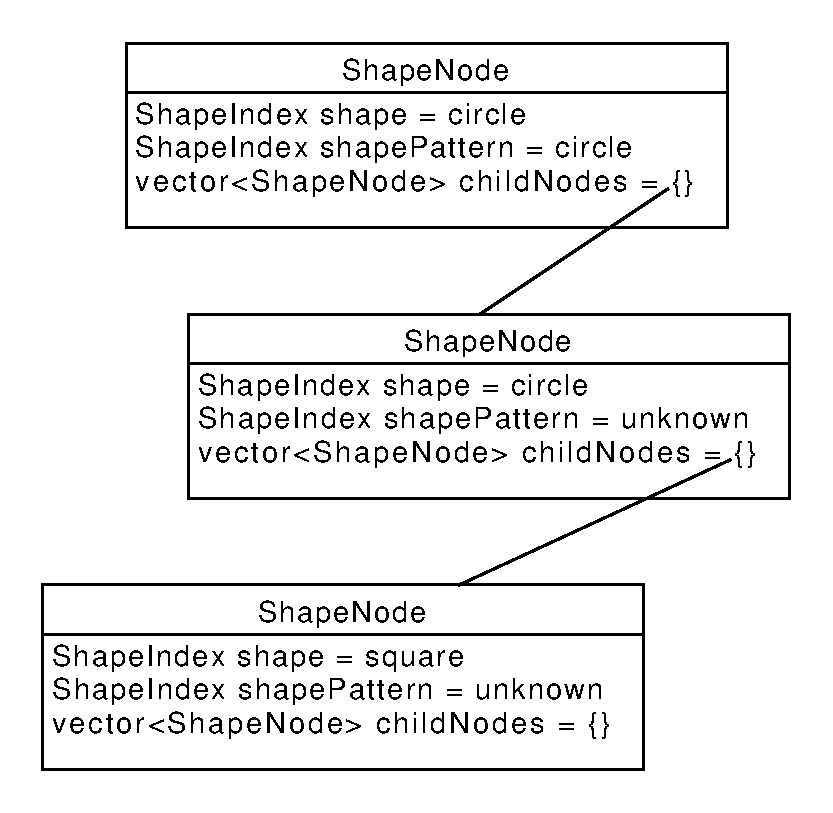
\includegraphics[width=.3\linewidth]{ext/images/example_output1.pdf}
\caption{The output schema for a more complicated image. }
\label{fig:output1}
\end{figure}


\end{description}

\section{Recognition process}
The recognition process is depicted in \cref{fig:algoschema}. It starts in the \texttt{Analyze} method, declared in the \texttt{ImageAnalyzer.h} file. It accepts an instance of \texttt{ImageLines} class as an argument, and returns \texttt{ShapeNode} instance describing the recognized elements in the image.

We have then decided to create the interface for the vector graphics form of input. We expect the input to the program to represent rather simple black and white shapes or their combinations, without any additional information like color or different shades. We also expect the input to be created on the computer in a game, rather than from a photo, and in this environment, it is common to use vector graphics.

\begin{figure}[p]
\centering
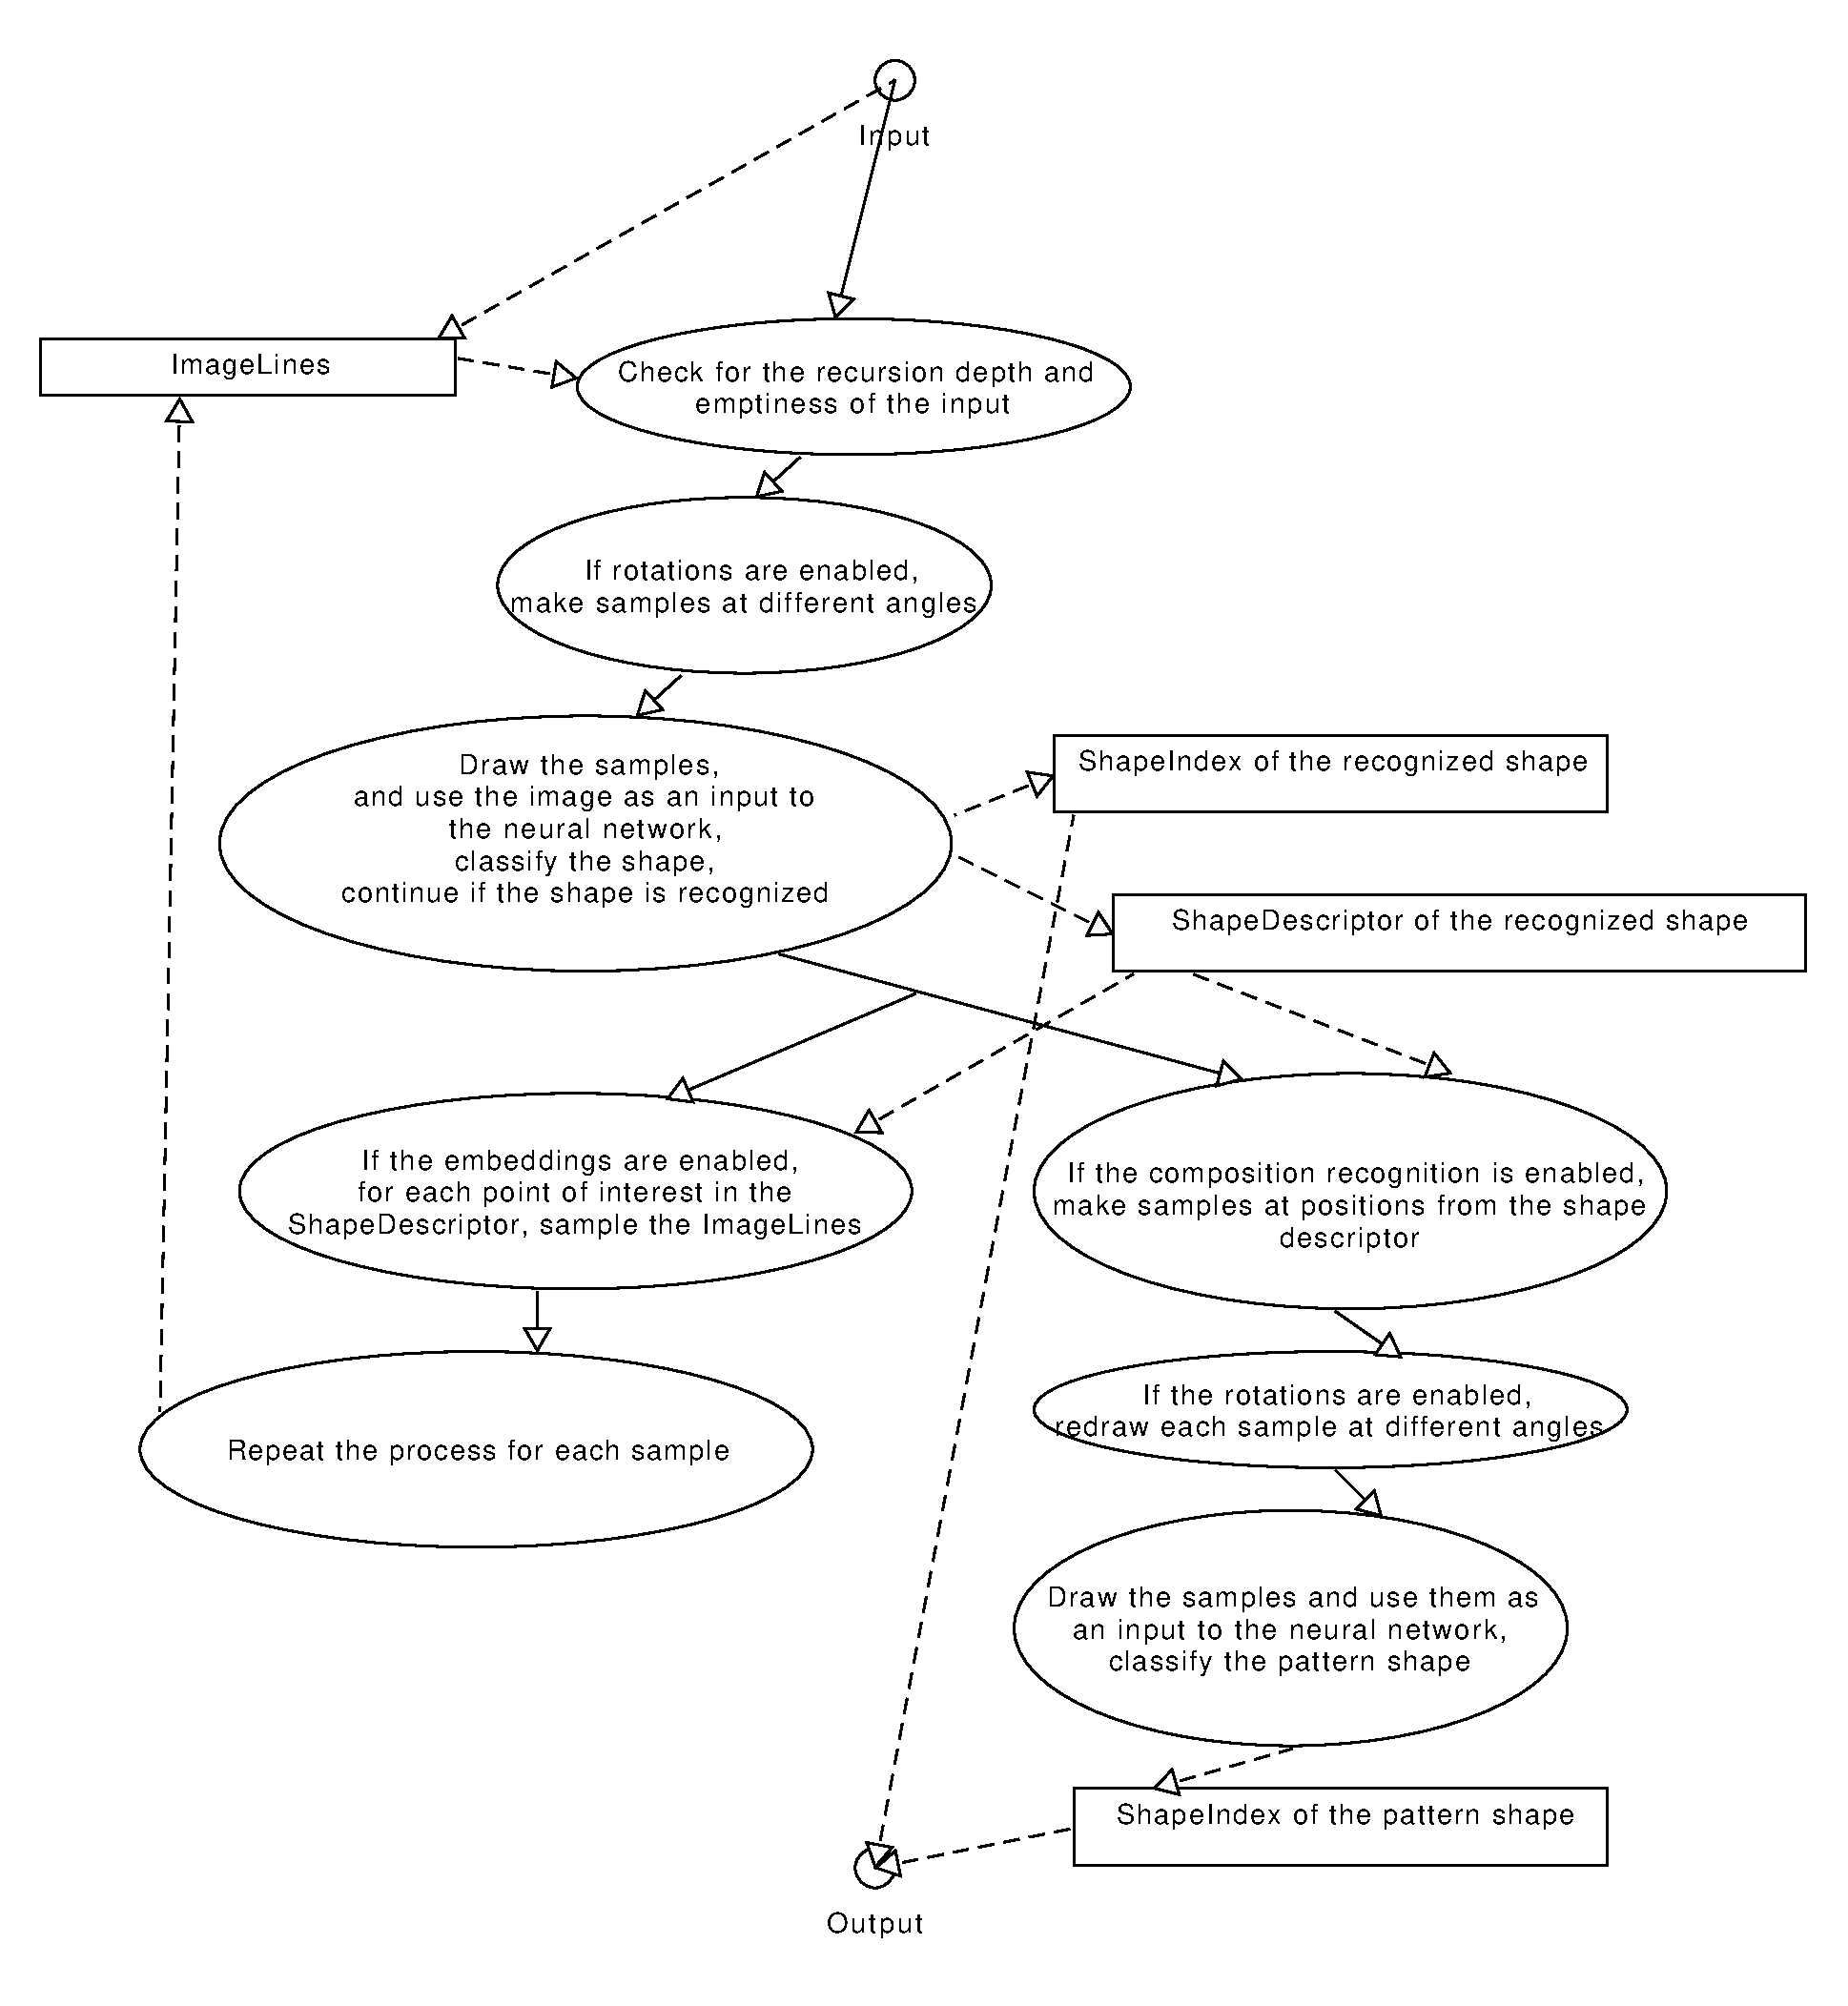
\includegraphics[width=.9\linewidth]{ext/images/algoschema.pdf}
\caption{The figure shows a general algorithm schema. The dashed arrows show appearances of important data structures: \texttt{ImageLines}, \texttt{ShapeIndex} and \texttt{ShapeDescriptor}. The full lines describe the algorithm flow. The algorithm starts with the input, the output is built during the analysis. The algorithm stops when the shape is not recognized.}
\label{fig:algoschema}
\end{figure}

The image lines are first normalized by normalization to the $[0-1]^2$ coordinate space. This transformation is essentially a rescaling, preserving both the length ratios and angles. Then, the top level shape is analyzed by rasterizing the lines into the pixel map which is then passed into the trained neural network.

Generally, the highest neural network output considered to be the matched shape pattern, but only if the value is higher than a user-set constant. There are optionally several more steps involved, described below:

\begin{description}
\item [Rotated shapes] If a recognition of rotated shapes is enabled, the image lines are rotated several times (the exact number is definable by user) by an appropriate angle value, re-drawn and analyzed by the network at each angle.

The network returns a vector of values, each output's value signaling the similarity to the shape assigned to the output, and the highest value is considered the matched shape. If there are several highest network outputs for different rotations with the same value, the first highest value among all outputs is considered. A recognized shape index is returned along with its matching rotation, in which it scored the highest network output.

\item[Composed shape]
When the top level shape is recognized, its shape descriptor is used to sample the theoretical curve points via parameter $t$ uniformly on interval $[0-1]$. If the recognition of rotated shapes is enabled, we transform the sample by an inverse rotation to the matched rotation, to align the recognized shape with the shape descriptor. Then, for each sampled point, this point is expanded into a small square, the original image is clipped to this square, discarding the lines outside, and the result is analyzed. 

Recognized pattern shapes are counted over all samples, and if the count of matches for any shape is high enough, the top level shape is recognized as a composed shape created from a number of smaller shapes of the type with the highest count. Pattern shapes that form the composition are not tested for embedded shapes.

\item [Embedded shape]
To recognize embedded shapes, we use the shape descriptor of the shape recognized previously, and focus on the user-defined embedded shape locations. For each embedded shape location defined in the shape descriptor, we clip the image lines to that area, and recursively run the \texttt{Analyze} method on the result. If the recognition of rotated shapes is enabled, we transform the an area by inverse rotation to the matched rotation, to align the recognized shape with the shape descriptor.
\end{description}

\section{Neural network preparation}
We use the \citet{fann} to train and use neural networks. This open source software is easy to use and install while having a lot of options in terms of network architecture and training. Thanks to its simple interface, we were able to develop an automatized training system for the networks.

\subsection{Training data}
Training the neural network requires a training dataset. Since we want to allow the extensibility in the form of user defined shapes, we have two options. Either to let the user somehow make his own dataset, which is not very convenient, or generate the data procedurally and try to approximate human-like drawing.

We decided for the second option. We generate the data based on the shape descriptors registered by the user and on the algorithm settings. To generate a data sample for the neural network, we take the shape descriptor and create a \texttt{ImageLines} instance from it.

Based on the algorithm settings, it will be either a deformed simple shape instance or an instance of a compound shape. In the case of creating a deformed simple shape, shape curve is sampled many times using the shape descriptor, and the points are connected by lines.
 
To approximate the deformations each point sample can be moved in the direction perpendicular to the line between the original position of the last point, and the original position of the the transformed point. Examples of deformations created by this procedure can be seen in \cref{deformed}.

\begin{figure}
\centering
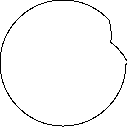
\includegraphics[width=.3\linewidth]{ext/images/deformed0.png}
\quad
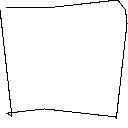
\includegraphics[width=.3\linewidth]{ext/images/deformed1.png}
\quad
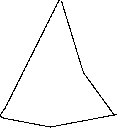
\includegraphics[width=.3\linewidth]{ext/images/deformed2.png}

\caption{Examples of generated deformations of the shapes.}
\label{deformed}
\end{figure}

The transformation  offset is linearly magnified and then reduced, resulting in a heuristics that try to approximate some of the humans like deformations of drawn shapes. Then, the line between the previous and new point is added to the image instance. 

In the case of the shape conglomeration, the shape curve is sampled less frequently and each point is replaced by rescaled image lines of a randomly chosen shape, but this shape is the same for the whole composition. See \cref{fig:examples} for examples.

\subsection{Training}
Training is done using the generated data from the previous methods and the \emph{FANN} library. 
First, the training data and test data are generated,The size of the test data is one-third of the size of training data. Then the network is repeatedly trained on the training data until it reaches the user set up MSE, or until it stops improving.

Internally, the training starts with a high MSE target value, which is then gradually lowered, and in between the improvement ratio is checked. We use the resilient backpropagation (rprop) algorithm from the FANN library, because we achieved best results with this algorithm in terms of the improvements stability. In the neural network, we use an \emph{Elliot} activation function \footnote{The Elliot activation function is:
	$y = \frac {\frac{(x*s)}{2}} {1+\abs{x*s})+ 0.5}$, where $s$ is the steepness parameter.
}.

\section{Game prototype}
The game, which demonstrates the usage of this pattern recognition work, has been developed using the \citet{urho} game engine in version 1.7. Urho3D is, as stated by authors, a free, lightweight, cross-platform 2D and 3D game engine implemented in C++ and released under the MIT license.

\subsection{Game description}
In the game, the player controls the character from a top down view perspective. The player can move and attack the enemies, and, most importantly, cast spells by drawing.

Spells of the game are represented by totem objects --- each time the player casts spell, a totem is created. These totem have different effects on the characters. They can take a form of positive effects that affect the player's character, like healing, or negative effects that affect the enemies, like burning. The task for the player is to survive and destroy all the enemies in the game.

We now describe some of the constructs of the game implementation:

\begin{description}
\item [Drawable texture] \texttt{DrawableTexture} is a component attached to ground in the game. It allows player to draw shapes onto the ground. This component handles the lines sampling and glowing shape line nodes, depicted in \cref{fig:drawing}.

\item [Characters] The player's character and the enemies \ref{fig:start} are represented by a composition of several components: the animated mutant model component, the health component and movement component. The enemies have also an AI component attached, while the player's character has an controller component attached which causes it to listen to the keyboard controls, and the caster component, which allows the character to extract drawn shape from the drawable texture, like in \cref{fig:square}. the caster component also transforms the shape into an \texttt{ImageLines} instance for the recognition.

\item [SpellSystem] The \texttt{SpellSystem} component is a initialization component for the recognition algorithm. It is created only once for the game and the algorithm setup is situated in the constructor. It holds the shape indexes and is responsible for the algorithm output parsing and construction of the spell.

\item [Spell] An instance of a node with the spell component is created each time the player casts a spell. It is a temporary class, serving as a placeholder for the totem object. It invokes the algorithm's \texttt{Analyze} method in a separate thread and waits for the result. This way, the game doesn't freeze while the algorithm analyzes the image. The place of the totem is marked by a green fire, as shown in \cref{fig:orb}, while the image is analyzed. 

\item [Totem] The core of the game are totem objects (see \cref{fig:totem}) and all the spell effects are represented by them. Each totem has a duration for which it exists and an area of effect around it, where the characters are influenced by its presence. The totem can have several effects to it attached. 

\item [Effects]  Effects are components attached to the totems. When a character is inside an area of effect of the totem, the totem applies all of its effects on the character. However, the effects can also be of an single activation type, in which case they are activated only once when the totem is created. An example of such effect is an effect that increases the totem duration.

\item [States] When an effect with duration is applied onto the character, a state component is attached to it, as shown in \cref{fig:effect}. For example, when an over-time healing effect is applied onto a character, the healing state component is attached to the character for a given duration.

\end{description}

\subsection{Spell system}
The game spell system consists of several parts. The first is the \texttt{DrawableTexture} component, which is attached to the ground entity. This component is able to track players drawings and store them as lists of points, each list representing one continuous line.

When the player presses the button to cast the spell, the \texttt{Caster} component attached to their character extracts the lines in a rectangular area around the character and transforms them into the vector of lines. Then the instance of \texttt{Spell} class defined in the \texttt{SpellSystem.h} file is created. There, the \texttt{ImageAnalyzer::Analyze} method is finally called in a different thread and when the analysis is done, the result is parsed and the spell is cast.

\begin{figure}[p]
\centering
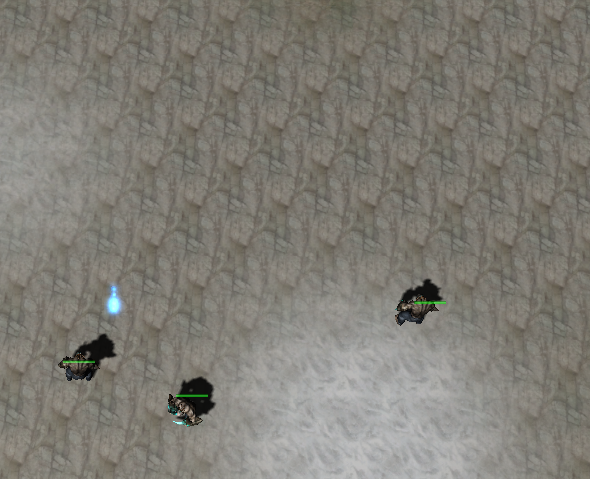
\includegraphics[width=.9\linewidth]{ext/scr/komix1.png}
\caption{There are three mutants in the image, one is controlled by the player, others are controlled by AI. The player starts drawing the spell on the ground by pushing the left mouse button. The mouse position is projected in the \texttt{Caster} component to the game surface and added to the \texttt{DrawableTexture} component which creates a new line.}
\label{fig:start}
\end{figure}

\begin{figure}[p]
\centering
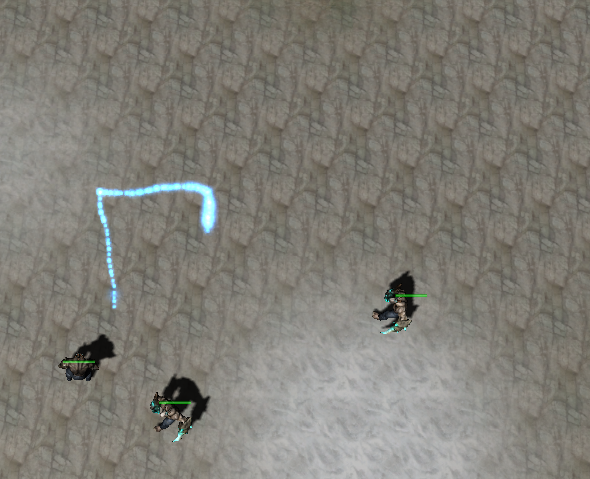
\includegraphics[width=.9\linewidth]{ext/scr/komix2.png}
\caption{The blue glowing line in the image represents the drawing. While the player holds the mouse button, the mouse positions are repeatedly sampled and projected to the surface. The projection points are then added to the line and the space between the points is filled with a blue glow dots to show the line. }
\label{fig:drawing}
\end{figure}

\begin{figure}[p]
\centering
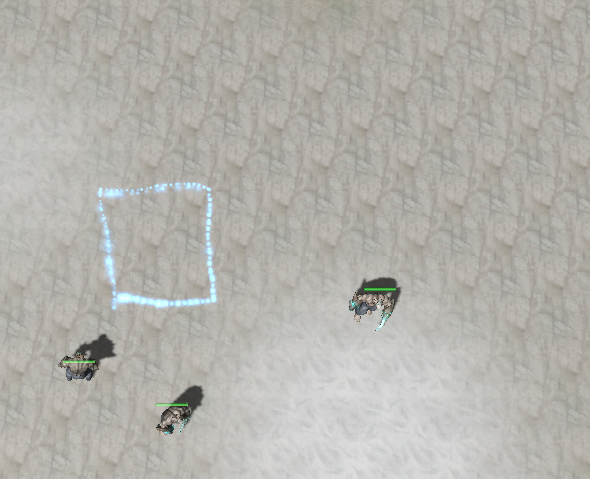
\includegraphics[width=.9\linewidth]{ext/scr/komix3.png}
\caption{The image shows a finished square shape. When the player releases the mouse, the current line is ended. It is possible to continue drawing other shapes. However, when the player casts spell, all lines in a large area around the character are consumed and used for the spell. The extraction of the lines from \texttt{DrawableTexture} and conversion into \texttt{ImageLines} class is done in the \texttt{Caster} component. }
\label{fig:square}
\end{figure}

\begin{figure}[p]
\centering
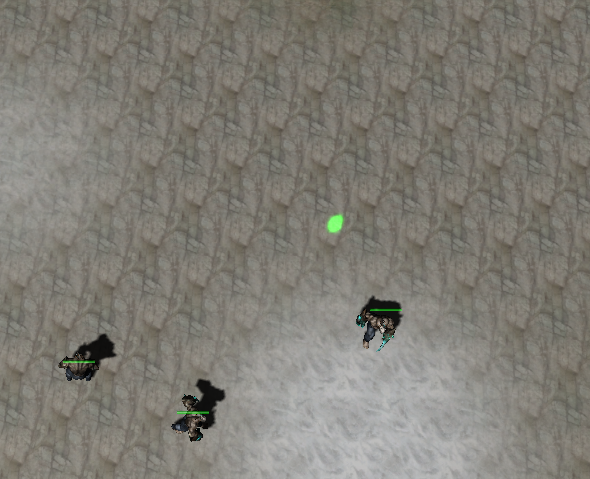
\includegraphics[width=.9\linewidth]{ext/scr/komix4.png}
\caption{When the player casts a spell, the extracted lines are removed and a node with the \texttt{Spell} component is created to handle the spell.  The node is represented by green glowing orb and it marks the place where the totem will be created. It invokes the \texttt{ImageAnalyer::Analyze} method with the lines in another thread to avoid the freezing while the analysis is performed. }
\label{fig:orb}
\end{figure}

\begin{figure}[p]
\centering
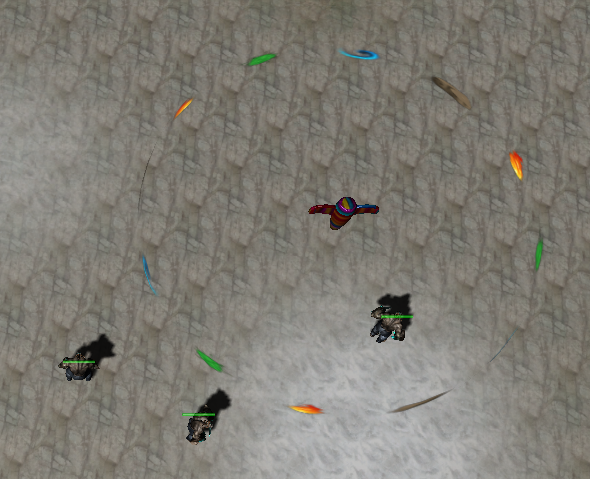
\includegraphics[width=.9\linewidth]{ext/scr/komix5.png}
\caption{When the analysis is finished, the \texttt{SpellSystem} component parses the output. It creates a node with the \texttt{Totem} component, and for each shape, the corresponding effect is added to the totem. The totem is then placed on the spot of the \texttt{Spell}. The totem's area of effect is marked by a rotating circle of elements. }
\label{fig:totem}
\end{figure}

\begin{figure}[p]
\centering
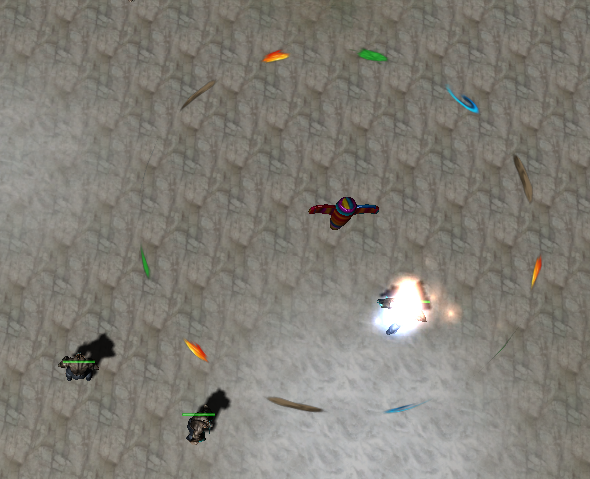
\includegraphics[width=.9\linewidth]{ext/scr/komix6.png}
\caption{The recognized shape was square. Since square represents fire, the totem has the \texttt{FireEffect} component attached to it. When the characters are detected inside the area of effect, the totem applies all of its effect on them. In the figure, the \texttt{FireEffect} is applied to the enemy inside the circle, causing it to have \texttt{FireState} component attached. This component makes the enemy burn, periodically decreasing its health.}
\label{fig:effect}
\end{figure}